%CS4099 Dissetation
%!TEX root = ../Project.tex
\section{Questionnaire}
% \label{Questionnaire}
\subsection{Task}

The task involves creating a single level of a Tactical RPG (Each level is grid based (like chess) where each player takes turns to move and/or attack the opposing player).   

\subsubsection*{Weapons}
\begin{center}
\begin{tabular}{c|c|c|c|}
	Name        & Weapon Type & Strength & Icon \\\hline
	Long Bow    & Ranged      & 30       & 
\includegraphics[height=0.5cm]{figures/bow.png}   \\ 
	Black Spear & Spear       & 20       & 
\includegraphics[height=0.5cm]{figures/spear.png} \\ 
	Ice Sword   & Melee       & 10       & 
\includegraphics[height=0.5cm]{figures/sword.png} \\ 
\end{tabular}
\end{center}

\subsubsection*{Skills}
\begin{center}
	\begin{tabular}{c|c|c|c|c}
		
		Name          & Type   & Range & Area & Strength \\\hline
		Thunder Flare & Ranged & 4     & 1    & 15       \\ 
	 	Air Blade     & Ranged & 2     & 0    & 25       \\ 
	\end{tabular}
\end{center}


% Makes a unit
\newcommand{\unit}[7]{\begin{tabular}{|p{1cm}|lp{2cm}|}
\hline
\multicolumn{3}{|c|}{#1} \\
\hline
\multirow{6}{*}{\includegraphics[height=1.7cm]{figures/#2}} 
 & Weapon    & #3 \\
 & Strength  & #4 \\
 & Move      & #5 \\
 \cline{2-3}
 & \multicolumn{2}{c|}{Skills} \\
 \cline{2-3}
 \ifstrempty{#6}{}{\foreach{\unitSkill}{}{#6}}
 & \multicolumn{2}{l|}{#7}\\
\hline
\end{tabular}
}

\newcommand\unitSkill[2]{
	& \multicolumn{2}{l|}{#2}\\
}
\subsubsection*{Units}
\unit{Agrias}{unit1.png}{Long Bow}{20}{3}{}{Air Blade}
\hspace{0.5cm}
\unit{Elena}{unit4.png}{Black Spear}{30}{5}{}{Thunder Flare}

\subsubsection*{Map Enemies}
\unit{Mustadio}{unit2.png}{Long Bow}{20}{3}{}{}
\hspace{0.5cm}
\unit{Druksmald}{unit3.png}{Ice Sword}{30}{5}{}{}
\\[0.5cm]
\unit{Zalbaag}{unit3.png}{Ice Sword}{25}{5}{}{}
\hspace{0.5cm}
\unit{Ajora}{unit3.png}{Ice Sword}{20}{5}{}{}


\clearpage
\subsubsection*{Map}
\begin{figure}[h!]
	\centering
		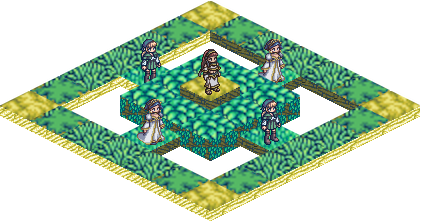
\includegraphics[height=2.7in]{figures/Task.pdf}
	\caption{The map to create}
	\label{fig:figures_Task}
\end{figure}


\paragraph{Win Condition\\}
Defeat Specific Unit   -- Elena.

\paragraph{Start Dialog:}
\begin{itemize}[topsep=0mm,noitemsep]
	\item[Text]  You can not Win!
	\item[Speaker] Kyou
\end{itemize}

\paragraph{End Dialog:}
\begin{itemize}[topsep=0mm,noitemsep]
	\item[Text]  How did I lose?
	\item[Speaker] Elena
\end{itemize}

\paragraph{Music:\\}
Background Music 3-15 Faraway Heights

\clearpage
\subsection{Editor Usability Scale}
% TODO ref this
{\footnotesize © Digital Equipment Corporation, 1986.}\\

\startingQuestion{I think that I would like to use this system frequently.}

\question{I found the system unnecessarily complex.}

\question{I thought the system was easy to use.}

\question{I think that I would need the support of a technical person to be able to use this system.}

\question{I found the various functions in this system were well integrated.}

\question{ I thought there was too much inconsistency in this system}

\question{ I found the system very cumbersome to use}

\question{ I felt very confident using the system}

\question{  I needed to learn a lot of things before I could get going with this system}

\subsection{Playing a pre-created game}

\startingQuestion{I found the game intuitive}

\question{The game had a appropriate level of difficulty. }

\question{I enjoyed playing the game.}

\fquestion{Please share any comments about the game :}


\clearpage
\subsection{Questions}
\fquestion{Have you played a Tactical RPG before?}

\fquestion{Did Engine have features you like to create in a game?}

\fquestion{How easy to use was the Engine?}

\fquestion{What particular aspects of the Engine did you like?}

\fquestion{What particular aspect of the Engine did you dislike?}

\fquestion{What features would you like to see added to the Engine in the future?}

\fquestion{Please share any other comments:}


